\documentclass[conference]{IEEEtran}
\IEEEoverridecommandlockouts
% The preceding line is only needed to identify funding in the first footnote. If that is unneeded, please comment it out.
\usepackage{cite}
\usepackage{amsmath,amssymb,amsfonts}
\usepackage{algorithmic}
\usepackage{graphicx}
\usepackage{textcomp}
\usepackage{xcolor}
\def\BibTeX{{\rm B\kern-.05em{\sc i\kern-.025em b}\kern-.08em
    T\kern-.1667em\lower.7ex\hbox{E}\kern-.125emX}}
\begin{document}

\title{Sensor Nodes Laboratory -- Final Report}

\author{\IEEEauthorblockN{Sebastian Thomas Thekkekara, Nitish Nagesh, Michael Haider, and Markus Becherer}
\IEEEauthorblockA{TUM Department of Electrical and Computer Engineering, Technical University of Munich, Munich, Germany \\
sebastian.thekkekara@tum.de, nitish.nagesh@tum.de, michael.haider@tum.de, and markus.becherer@tum.de}
}

\maketitle

\begin{abstract}
Temperature sensors play an important role in domestic and industrial applications. Measuring data in specific intervals is useful in analyzing the trends. Temperature data was sent to the PSoC at two second intervals. A second order butterworth low-pass filter using sallen-key topology was designed to send appropriate frequency samples to analog-to-digital converter (ADC). UART communication protocol was used to communicate betwwen Ardunio and Programmable-System-on-Chip (PSoC) integrated development environment (IDE). Inter-integrated-circuit (I2C) communication protocol was used to communicate between the arduino and the launchpad . The temperature data was encapsulated, enqueued and sent wirelessly over a server to a receiver. The data was observed on a terminal in a remote location. Fallback strategies and scaling-up method are discussed to enable widespread use of wireless sensor nodes.
\end{abstract}

\begin{IEEEkeywords}
temperature data, PSoC, CC1350 Launchpad, I2C, UART
\end{IEEEkeywords}

\section{Introduction}
The number of connected devices are increasing rapidly. The internet has brought a revolution ushering in renewed enthusiasm for staying connected while transcending geographical and temporal boundaries. Internet of Things (IoT) is a field which enables devices to be connected over the internet. IoT is the basis for applications such as smart homes, smart vehicles, smart meters, smart grids and so on. Each of these applications uses sensors to measure parameters such as temperature, humidity, pressure, emissions etc. which are activated based on various stimuli. These parameters are continuously monitored and in a feedback loop while checking for threshold values. Based on the operating conditions and algorithm used, specific actions can be taken to utilize sensor data. In the end, a database is available which can be used for future reference and can also be utilized for training neural networks enabling better data analysis and easier anomaly detection in case of wide deviations from reference values.

In this project, we intend to mimic an industrial workflow to develop a prototype from a given set of components and tools. The goal is to develop a fully functional prototype of a wireless sensor node by the end of summer semester 2019 i.e. September 2019. A resistance temperature detection (RTD) sensor Pt1000 is provided, along with PSoC 5LP (Programmable System-on Chip) and Texas Instruments CC1350 Launchpad. The aim is to measure the surrounding temperature every two seconds using the temperature sensor provided and display the output on a terminal. A fallback plan is also devised in case data measurements are insufficient or inappropriate. The project is divided into sub-tasks and illustrated accordingly for logical and streamlined workflow. They include:
\begin{itemize}
	\item Developing a read-out front-end circuit 
	\item Implementing a communication interface between the read-out circuit and wireless communication board
	\item Encapsulating the data, sending it over a server and visualizing it on a terminal
\end{itemize}
 This would contribute to the already existing connected devices and in-turn facilitate smoother implementation in various applications.
 
 \section{Block Diagram}
\begin{figure}
	\centering
	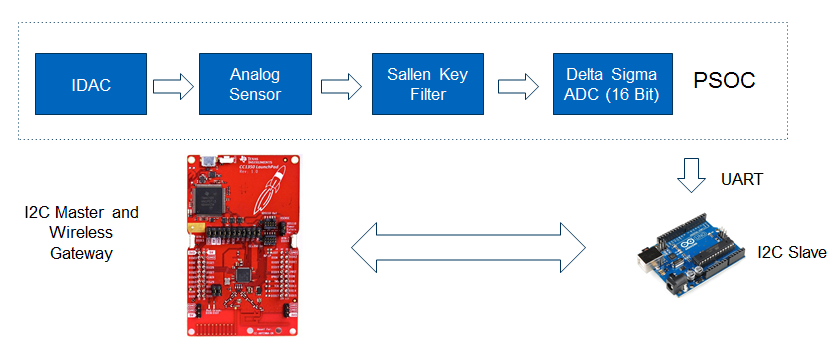
\includegraphics[width=1\linewidth, height=0.2\textheight]{00_block_diagram}
	\caption{}
	\label{fig:00blockdiagram}
\end{figure}

%\begin{figure}[htbp]
%	\centerline{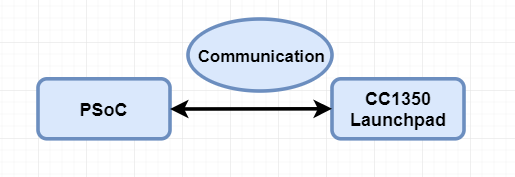
\includegraphics[width=\columnwidth]{00_rx_1}}
%	\caption{Receiver}
%	\label{fig:rx}
%\end{figure}

Fig. \ref{fig:00blockdiagram} shows the block diagram of the transmitter and receiver of the project setup. In the transmission side, a current is supplied from the current digital-to-analog converter (IDAC) and then sent to the RTD Pt1000 temperature sensor. A filter is designed to provide near noise-free signals to the in-built ADC in the PSoC. A communication is established between the CC1350 Launchpad and PSoC using standard communication protocols. The temperature data is read at regular intervals and sent to a remote receiver.

\section{Analog Front End}

In the first few weeks, we spent time on understanding the basics of Analog-to-Digital Converters (ADCs), different types of filters and filter design principles. We also installed PSoC Creator 4.2 by Cypress Semiconductors and Code Composer Studio (CCS) by Texas Instruments (TI). The lectures gave us an overview about the filter design and analog interface. We were also briefed about the different types of communication protocols which could used to transmit data. We initially tried to develop a basic block diagram and read application notes related to temperature measurement using RTD in PSoC Creator. Different RTD configurations were available such as 2-wire, 3-wire and 4-wire configurations. 3-wire and 4-wire configurations allowed higher accuracy of resistor measurements by eliminating voltage drop across the lead connections and taking the voltage purely across the RTD for measurement \cite{b1}. We chose the 2-wire configuration for the sake of simplicity. To measure the resistance accurately, the current source and the ADC measuring the voltage must be accurate. There is a possibility to include a reference resistor to minimize the gain/offset error caused by the Analog-to-Digital Converter (ADC) and the Current Digital to Analog Converter (IDAC). The current passed through the RTD was taken as 1 mA. The value of current is chosen such that it does not cause self-heating across RTD while still ensuring that the maximum range of the ADC can be used. 

A preliminary design involving IDAC, RTD and ADC was first developed. An Arduino was first used as the wireless board and the temperature data was sent to it using Universal Asynchronous Receiver Transmitter (UART) protocol. The output was viewed on a terminal. The process required multiple iterations and rewiring before the output was obtained. It was interesting to note that values of the datatype float were not displayed on the terminal and only values of type integer were displayed. In the next step, a filter was designed to supply filtered output to the ADC. 

\begin{figure}[htbp]
	\centerline{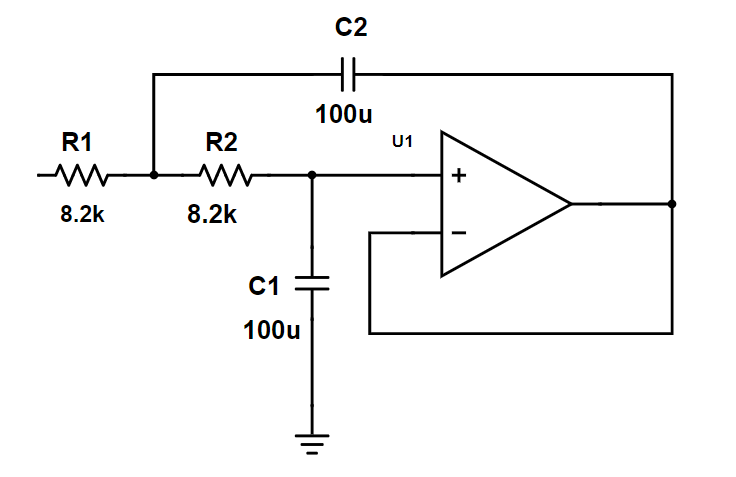
\includegraphics[width=\columnwidth, height=0.3\textheight]{06_sallen_key_filter}}
	\caption{Second order low-pass butterwoth filter using sallen-key topology}
	\label{fig:filter}
\end{figure}

For this purpose, a low pass filter was used as shown in Fig. \ref{fig:filter} with quality factor Q = 1/2. The temperature data is read every 2 seconds which corresponds to 0.5 Hz. According to the Nyquist criteria, the filter was designed such that its maximum cut-off frequency of the filter is the ADC sampling frequency/2 i.e. 0.25 Hz. To maintain anti-aliasing effect, we chose the cut-off frequency f\textsubscript{c} as 0.2 Hz. A second order butterworth low pass filter was implemented using sallen-key topology as it is an active filter topology. Using \cite{b2}, the two resistance values were chosen as 8.2 k$\Omega$ and the two capacitance values were chosen as 100 $\mu$F. 

Fig. \ref{fig:afc} shows the schematic in PSoC for implementing the temperature sensor. The IDAC is supplying current to a 1000 $\Omega$ resistor. Then, the filter is connected which is later connected to ADC. Pulses are triggered to the ADC at regular intervals and communication is setup with the launchpad.
\begin{figure}[htbp]
	\centerline{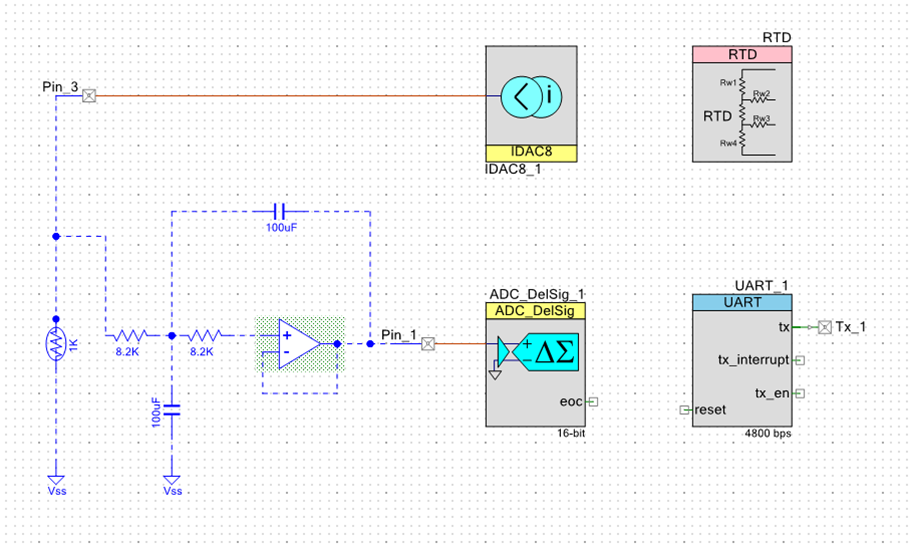
\includegraphics[width=\columnwidth, height=0.3\textheight]{04_psoc_with_filter}}
	\caption{PSoC schematic}
\label{fig:afc}
\end{figure}


\section{Communication Interface}

After designing the filter, we established the interface between the PSoC, off-chip components including RTD and filter, and the CC1350 Launchpad via a communication protocol. This process as well had its share of challenges. We first tried implementing I2C communication using Arduino. The process was straightforward with using the Arduino as the master and a slave in the PSoC with SDA being used to transmit or receive serial data and SCL being the master generated clock. When we started implementing the same I2C protocol on the CC1350 Launchpad, we were not able to load the program even after building it due to missing libraries. After updating the drivers and rewiring the connections, the output was erratic. Finally, the launchpad had to be replaced with a new one before we could start tweaking the C code already provided.

The code was already provided to ensure compliance with the German laws such that data is transmitted only in the allowed and free band of 868 MHz. A deviation from this standard could result in interference with other communication and military frequency bands and is best avoided at all costs. As stated before, the temperature value is read every two seconds. The circuit is wired as shown in Fig. \ref{fig:comm}. A constant voltage of 5 V from the signal generator is applied across the IC741 operational amplifier (op-amp). The sallen-key filter designed is implemented which is then connected to the CC1350 Launchpad consisting the ADC. The voltage is measured across the Pt1000 by passing a current of 1 mA from the IDAC. It was observed that voltage is 1.113 V corresponding to a resistance of 1113 $\Omega$. This corresponds to a temperature of $30$\textdegree C \cite{b4}.

\begin{figure}[htbp]
	\centerline{\includegraphics[width=\columnwidth, height=0.3\textheight]{08_working_interface}}
	\caption{Wired circuit with temperature sensor, filter design and communication interface}
	\label{fig:comm}
\end{figure}

The I2C master triggers the ADC and the I2C slave on the PSoC responds based on the master clock signals. I2C allows multiple masters and slaves to be connected without disturbing the communication pathway. This is possible because I2C uses a unique address transmitted before sending the data and also has a shared bus allowing many devices to be connected at a time. As a result, I2C uses lesser number of wires and allows data transmission on a single while enabling lower pin count \cite{b3}. The ADC in the PSoC can be operated in either continuous or single sample mode. In single sample mode, the data is read at the intervals triggered by the master. In continuous mode, the data is read uninterrupted and code has to be changed to calculate cumulative value of temperature. Average value of the data is considered to eliminate effects of noise and ensure zero mean. In this project, since the temperature is read every two seconds, even if the ADC is operated in continuous mode, the sampling becomes unnecessary and is in effect equivalent to simple sampling implemented. 

 
\section{Data Encapsulation and Enqueuing }

Once the analog-front end was completed and the communication was setup with the CC1350 Launchpad, we started rewriting the code to obtain the temperature every two seconds. The I2C master was activated with a data rate of 400 kbps. The slave address in the PSoC was entered in the code so as to transmit data over the bus. The internal clock of the PSoC calculates the needed frequency of the I2C clock source and generates appropriate resources needed for its implementation. Pull-up resistors of 2.7 k$\Omega$ were used. This method did not generate the required result. We observed that PSoC was not able to read the data and send it to the buffer on CCS. We checked if it was an error with the launchpad. We wrote an I2C communication protocol between ardunio and CC1350 Launchpad and it worked well. We also used the oscilloscope to verify if signals were being received. After manipulating the C code in PSoC and CCS, we triggered the data pins on the launchpad. It was observed that the PSoC failed to read data and as a result, the response was not as desired.  %Even though the duty cycle available is 20 bytes per second, only two bytes are used in this project. 

We then tried implementing the UART communication protocol between the PSoC and launchpad. We were able to read temperature successfully on the terminal. Later, this was to be sent to a remote receiver and in this way, a wireless sensor node could be setup. But, we were not satisfied with this due to non-scalable nature of UART. UART uses one-on-one serial communication between two devices and does not allow addition of new devices to the set-up. This is a setback in practical applications which requires adaptation to new lines without much change in the hardware architecture.

To improve this design, we came up with a new idea. The main problem as highlighted before was that I2C communication was not successful between PSoC and CC1350 launchpad. However, the I2C communication between arduino and launchpad was working perfectly. Further, the communication between arduino and PSoC was not a problem. Therefore we decided to communicate between the PSoC and arduino using UART and between arduino and launchpad via I2C. This implementation is shown in Fig. \ref{fig:full}. The other aspects of the analog front-end were not changed.

\begin{figure}[htbp]
	\centerline{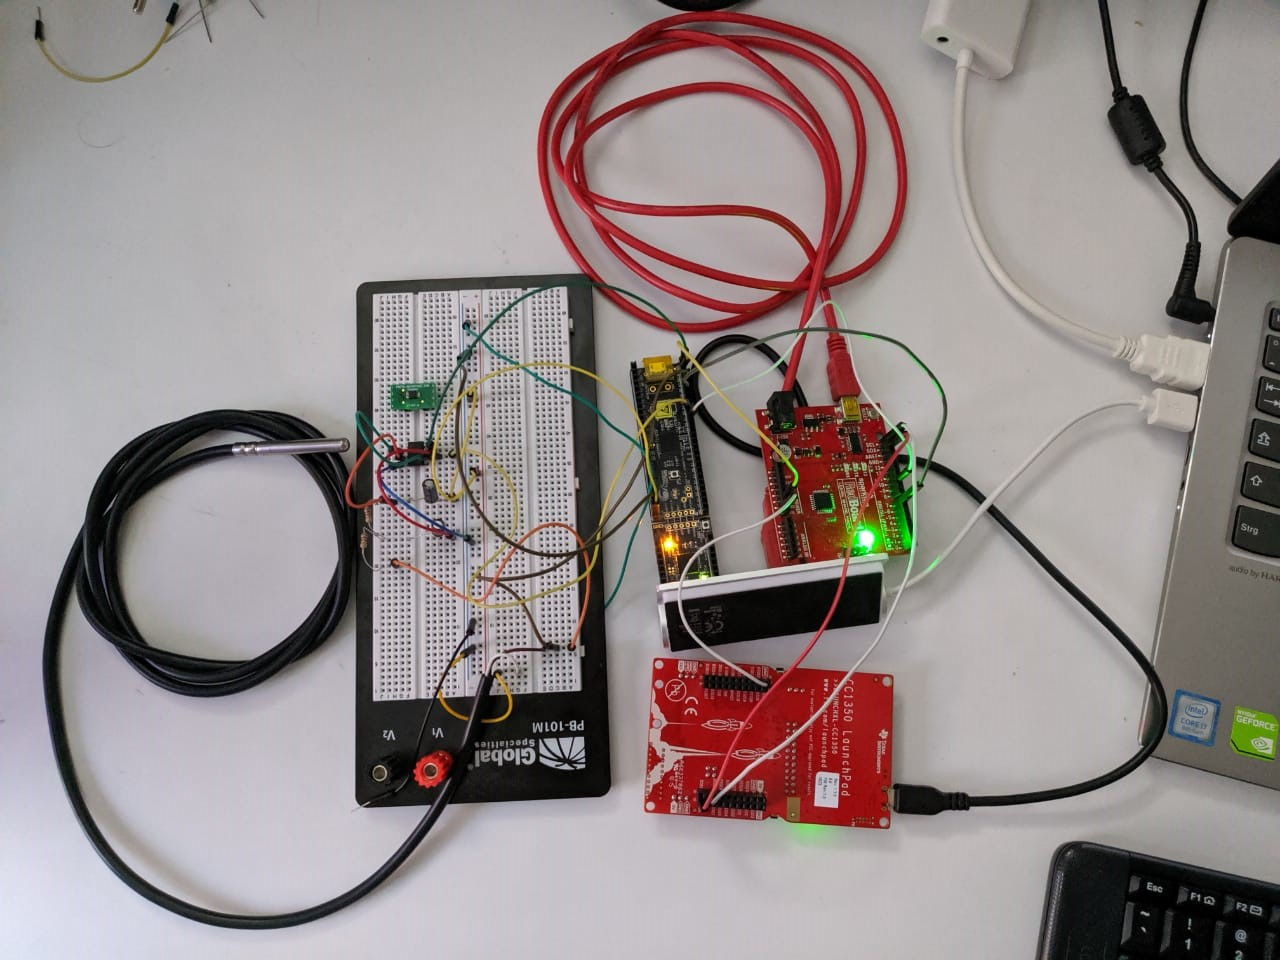
\includegraphics[width=\columnwidth, height=0.3\textheight]{07_full_circuit}}
	\caption{Working prototype}
	\label{fig:full}
\end{figure}


The data was enqueued on the bus and the resistance was calculated. The corresponding temperature was calculated according to the equation \cite{b5}
\begin{equation}
	R\textsubscript{T} = R\textsubscript{0} (1 + AT + BT\textsuperscript{2})
\end{equation}
 where 	R\textsubscript{T}  is the resistance at T \textdegree C and R\textsubscript{0} is resistance at $0$ \textdegree C. In our project R\textsubscript{0} is 1000 $\Omega$. 
 
 Equation 1 is valid for temperatures above $0$ \textdegree C.  For temperatures below $0$ \textdegree C \cite{b5}, equation 2 is used.
 \begin{equation}
 R\textsubscript{T} = R\textsubscript{0} (1 + AT + BT\textsuperscript{2} + C(T-100)T\textsuperscript{3})
 \end{equation}
 where 	R\textsubscript{T}  is the resistance at T \textdegree C and R\textsubscript{0} is resistance at $0$ \textdegree C. In our project R\textsubscript{0} is 1000 $\Omega$. 
 
  The RTD block in the PSoC was initially not working as intended. We set the temperature range from -50\textdegree C to 100\textdegree C in the RTD block. The coefficients A, B and C were automatically generated in PSoC and a maximum calculation error of 0.02\textdegree C was observed. In the end, we were able to utilize the full potential of the RTD block and implement it in our project.
 
 \section{Data Visualization}
 
The resistance calculated in m$\Omega$ is a two byte data.  This data is split into two components of one byte each and then transferred to the CC1350 Launchpad. Based on the calculated resistance value and coefficients, a quadratic relation from equation 1 and cubic relation from equation 2 between temperature and resistance is obtained.  In the launchpad, they are again combined to form a 16 bit value which is used to calculate the temperature. The corresponding values of resistance and temperature was compared with values in the look-up table \cite{b4}. It was found that there was only a slight deviation of both values when measurements were carried out at room temperature. One reason for the deviation can be attributed to interference from external noise. Another reason is the offset voltage between the inverting and non-inverting of the op-amp.
 
%The communication with I2C is also not ideal as some data is lost in the interface of communication and on the bus. 
After the temperature was calculated, it was transmitted wirelessly over the server. This was possible via a specific address internet protocol (IP) address assigned to the launchpad. Fig. \ref{fig:receiver} shows the data received in a remote location. In this way, we were able to complete all the tasks assigned and implement a fully functional wireless sensor node.
%Include new figure.
\begin{figure}[htbp]
	\centerline{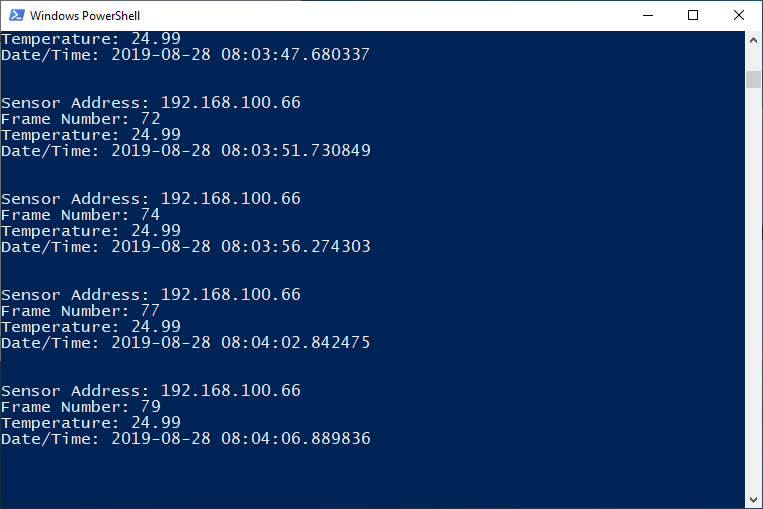
\includegraphics[width=\columnwidth, height=0.3\textheight]{temp_server}}
	\caption{Wireless data reception}
	\label{fig:receiver}
\end{figure}

\section{Fallback strategies and Scaling-up}
While implementing this project, we faced considerable challenges with respect to hardware and software tools. It is of utmost importance that the sensor data is available at regular intervals. If the temperature is not read every two seconds an alert can be generated requesting a trigger from the terminal manually. The program can also be modified such that the launchpad and connected devices are sent into sleep mode after actuation by an undesirable input. When normal operation is to be run, the I2C communication, for instance can be woken up form sleep mode. The IDAC current can also be supplied intermittently based on request. This also enables power saving.

Power saving is especially crucial while using sensor nodes for practical applications such as smart lighting, smart meters, home automation etc. It helps increase longevity of the device under use thereby contributing to significant cost saving in corporations and institutions. The I2C communication protocol enables easy scaling-up of the prototype due to the availability of multi-master slave. Additional sensors such as humidity, ambient light, pressure etc. can be added to the existing prototype by using current multiplexer (MUX) and ADC MUX. The code has to be modified appropriately and each parameter can be observed simultaneously. 

Once the data is received over a cloud to a terminal, different analysis methods such as artificial intelligence can be applied to understand data over a period of time. The communication can be made secure by upgrading security protocols. Deep learning algorithms can be implemented which will analyze temperature data trends and predict possible scenarios. This can be used for a variety of applications such as weather forecasting. 

\section{Conclusion}
Over the course of the semester, we learnt different aspects of a wireless sensor node and successfully built a prototype to read temperature data at regualar intervals. We utilized the hardware and software components provided and overcame challenges while implementing each of the sub-tasks assigned. We are now able to evaluate a sensor node in an IoT framework on both device and circuit level while applying it to a specific application.

\section*{Acknowledgment}

We thank Michael Haider for guiding us throughout the entire project. Michael helped us understand the basics required for completing the prototype along with providing the hardware components and software tools required to complete this project. He was available whenever requested and was instrumental in improving our understanding of developing a wireless sensor node. We sincerely thank professor Markus Becherer for giving us an opportunity to participate in this laboratory course and allowing access to labs at the chair which helped us work efficiently and effectively.


\begin{thebibliography}{00}
\bibitem{b1} http://www.cypress.com/AN70698
\bibitem{b2} http://sim.okawa-denshi.jp/en/OPstool.php
\bibitem{b3} https://maker.pro/arduino/tutorial/common-communication-peripherals-on-the-arduino-uart-i2c-and-spi
\bibitem{b4} Kongsberg Maritime AS, "Platinum resistance temperature sensors Pt100 (Pt1000)" .
\bibitem{b5} http://www.cypress.com/AN70698
%\bibitem{b6} Y. Yorozu, M. Hirano, K. Oka, and Y. Tagawa, ``Electron spectroscopy studies on magneto-optical media and plastic substrate interface,'' IEEE Transl. J. Magn. Japan, vol. 2, pp. 740--741, August 1987 [Digests 9th Annual Conf. Magnetics Japan, p. 301, 1982].
%\bibitem{b7} M. Young, The Technical Writer's Handbook. Mill Valley, CA: University Science, 1989.
\end{thebibliography}

%\bibliography{references}
\end{document}
